\documentclass[slovene,11pt,a4paper]{article}
\usepackage[margin=2cm,bottom=3cm,foot=1.5cm]{geometry}

\setlength{\parindent}{0pt}
\setlength{\parskip}{0.5ex}
\setlength{\emergencystretch}{1em}
\pagestyle{empty}

\usepackage[pdftex]{graphicx}
\graphicspath{{figs/}}

\DeclareGraphicsExtensions{.pdf,.png,.jpg}
\usepackage{amsmath}
\usepackage{amsfonts}
\usepackage{amssymb}
\usepackage[usenames]{color}
\usepackage[slovene]{babel}
\usepackage[utf8]{inputenc}
\usepackage[T1]{fontenc}

\usepackage{pythonhighlight}
\usepackage{tikz}
\usetikzlibrary{arrows.meta,babel}
\definecolor{bcol}{RGB}{217,95,2}
\definecolor{jetcol}{RGB}{49,130,189}
\definecolor{neucol}{gray}{0.55}
\usepackage{parskip}
\usepackage{hyperref}
\usepackage{lmodern}
\usepackage{tgschola}

%
\title{
\sc\large Praktikum strojnega učenja\\
\bigskip
\bf\Large 6.~naloga\\ Gručenje in označevanje hadronskih curkov
}
\author{}
\date{}


\begin{document}
\maketitle
\vspace{-1cm}

\section*{Kaj so hadronski curki}

Pri visoko-energijskih trkih med osnovnimi delci nastane veliko število delcev v končnem stanju, katerih fizikalne lastnosti, kot je energija, se lahko zaznajo s posebnimi detektorji. Med temi delci so pogosto prisotni hadroni, kot so proton, nevtron ali pion, ki jih pogosto zaznamo tudi v kozmičnih žarkih. Več primerov hadronov je na voljo na spletni strani Particle Data Group (PDG) \cite{pdg}, v sekcijah \textit{Mesons} (mezoni - hadroni s celoštevilskim spinom) in \textit{Baryons} (barioni - hadroni s polcelim spinom).

Danes je znano, da hadroni niso osnovni delci, temveč so sestavljeni iz kvarkov, ki jih veže močna interakcija. Standardni model je teorija osnovnih delcev, katere del je tudi kvantna kromodinamika (QCD, \textit{quantum chromodynamics}), ki opisuje močno interakcijo. Standardni model opisuje spekter osnovnih delcev in dinamiko med njimi, ne pa tudi eksplicitno vezanih stanj. To vodi do pomembnega vprašanja: kako povezati kvarkovska končna stanja s hadroni, ki jih zaznamo v eksperimentih? Prostih kvarkov namreč ni mogoče zaznati, saj se zaradi narave močne interakcije hitro vežejo v hadrone.

Poleg tega močna interakcija povzroči tudi sevanje gluonov - prenašalcev močne interakcije - iz kvarkov. Ti gluoni nato lahko tvorijo nove kvarke ali pa se vežejo v hadrone. Ta proces se lahko večkrat ponovi, kar v končnem stanju privede do velikega števila hadronov (hadronizacija), ki izvirajo iz nekaj kvarkov nastalih v osnovni interakciji, glej sliko \ref{fig:hadronization}. Hadroni so pogosto zelo kolimirani, kar pomeni, da je mogoče ločiti skupine hadronov, ki izvirajo iz enega kvarka, od drugih. Te skupine hadronov imenujemo hadronski curki (\textit{hadronic jets}).

Transformacija od kvarkov do končnih hadronskih curkov ne spremeni signifikantno informacij o energiji in gibalni količini, kar pomeni, da curke lahko uporabimo za študijo procesov v fiziki osnovnih delcev ter primerjavo s teorijo, četudi ta govori v jeziku kvarkov \cite{jetsSeymour:1995gq, jetbook}.

V primeru, ko v nekem procesu pričakujemo dva kvarka, se v eksperimentu načeloma pričakuje dva hadronska curka. Vendar pa bo v praksi število hadronskih curkov običajno večje, saj lahko tudi začetna stanja trkov, kot v primeru trkalnika LHC, sevajo gluone. S tem se celoten proces hadronizacije lahko ponovi tudi za te gluone, kar povzroči nastanek dodatnih hadronov v končnem stanju. To težavo običajno rešimo z uporabo filtriranja curkov na podlagi kinematičnih lastnosti, s ciljem obravnavati samo najbolj visokoenergijske curke, ki so najverjetneje povezani z osnovnim procesom.



\begin{figure}[htb]
	\centering
	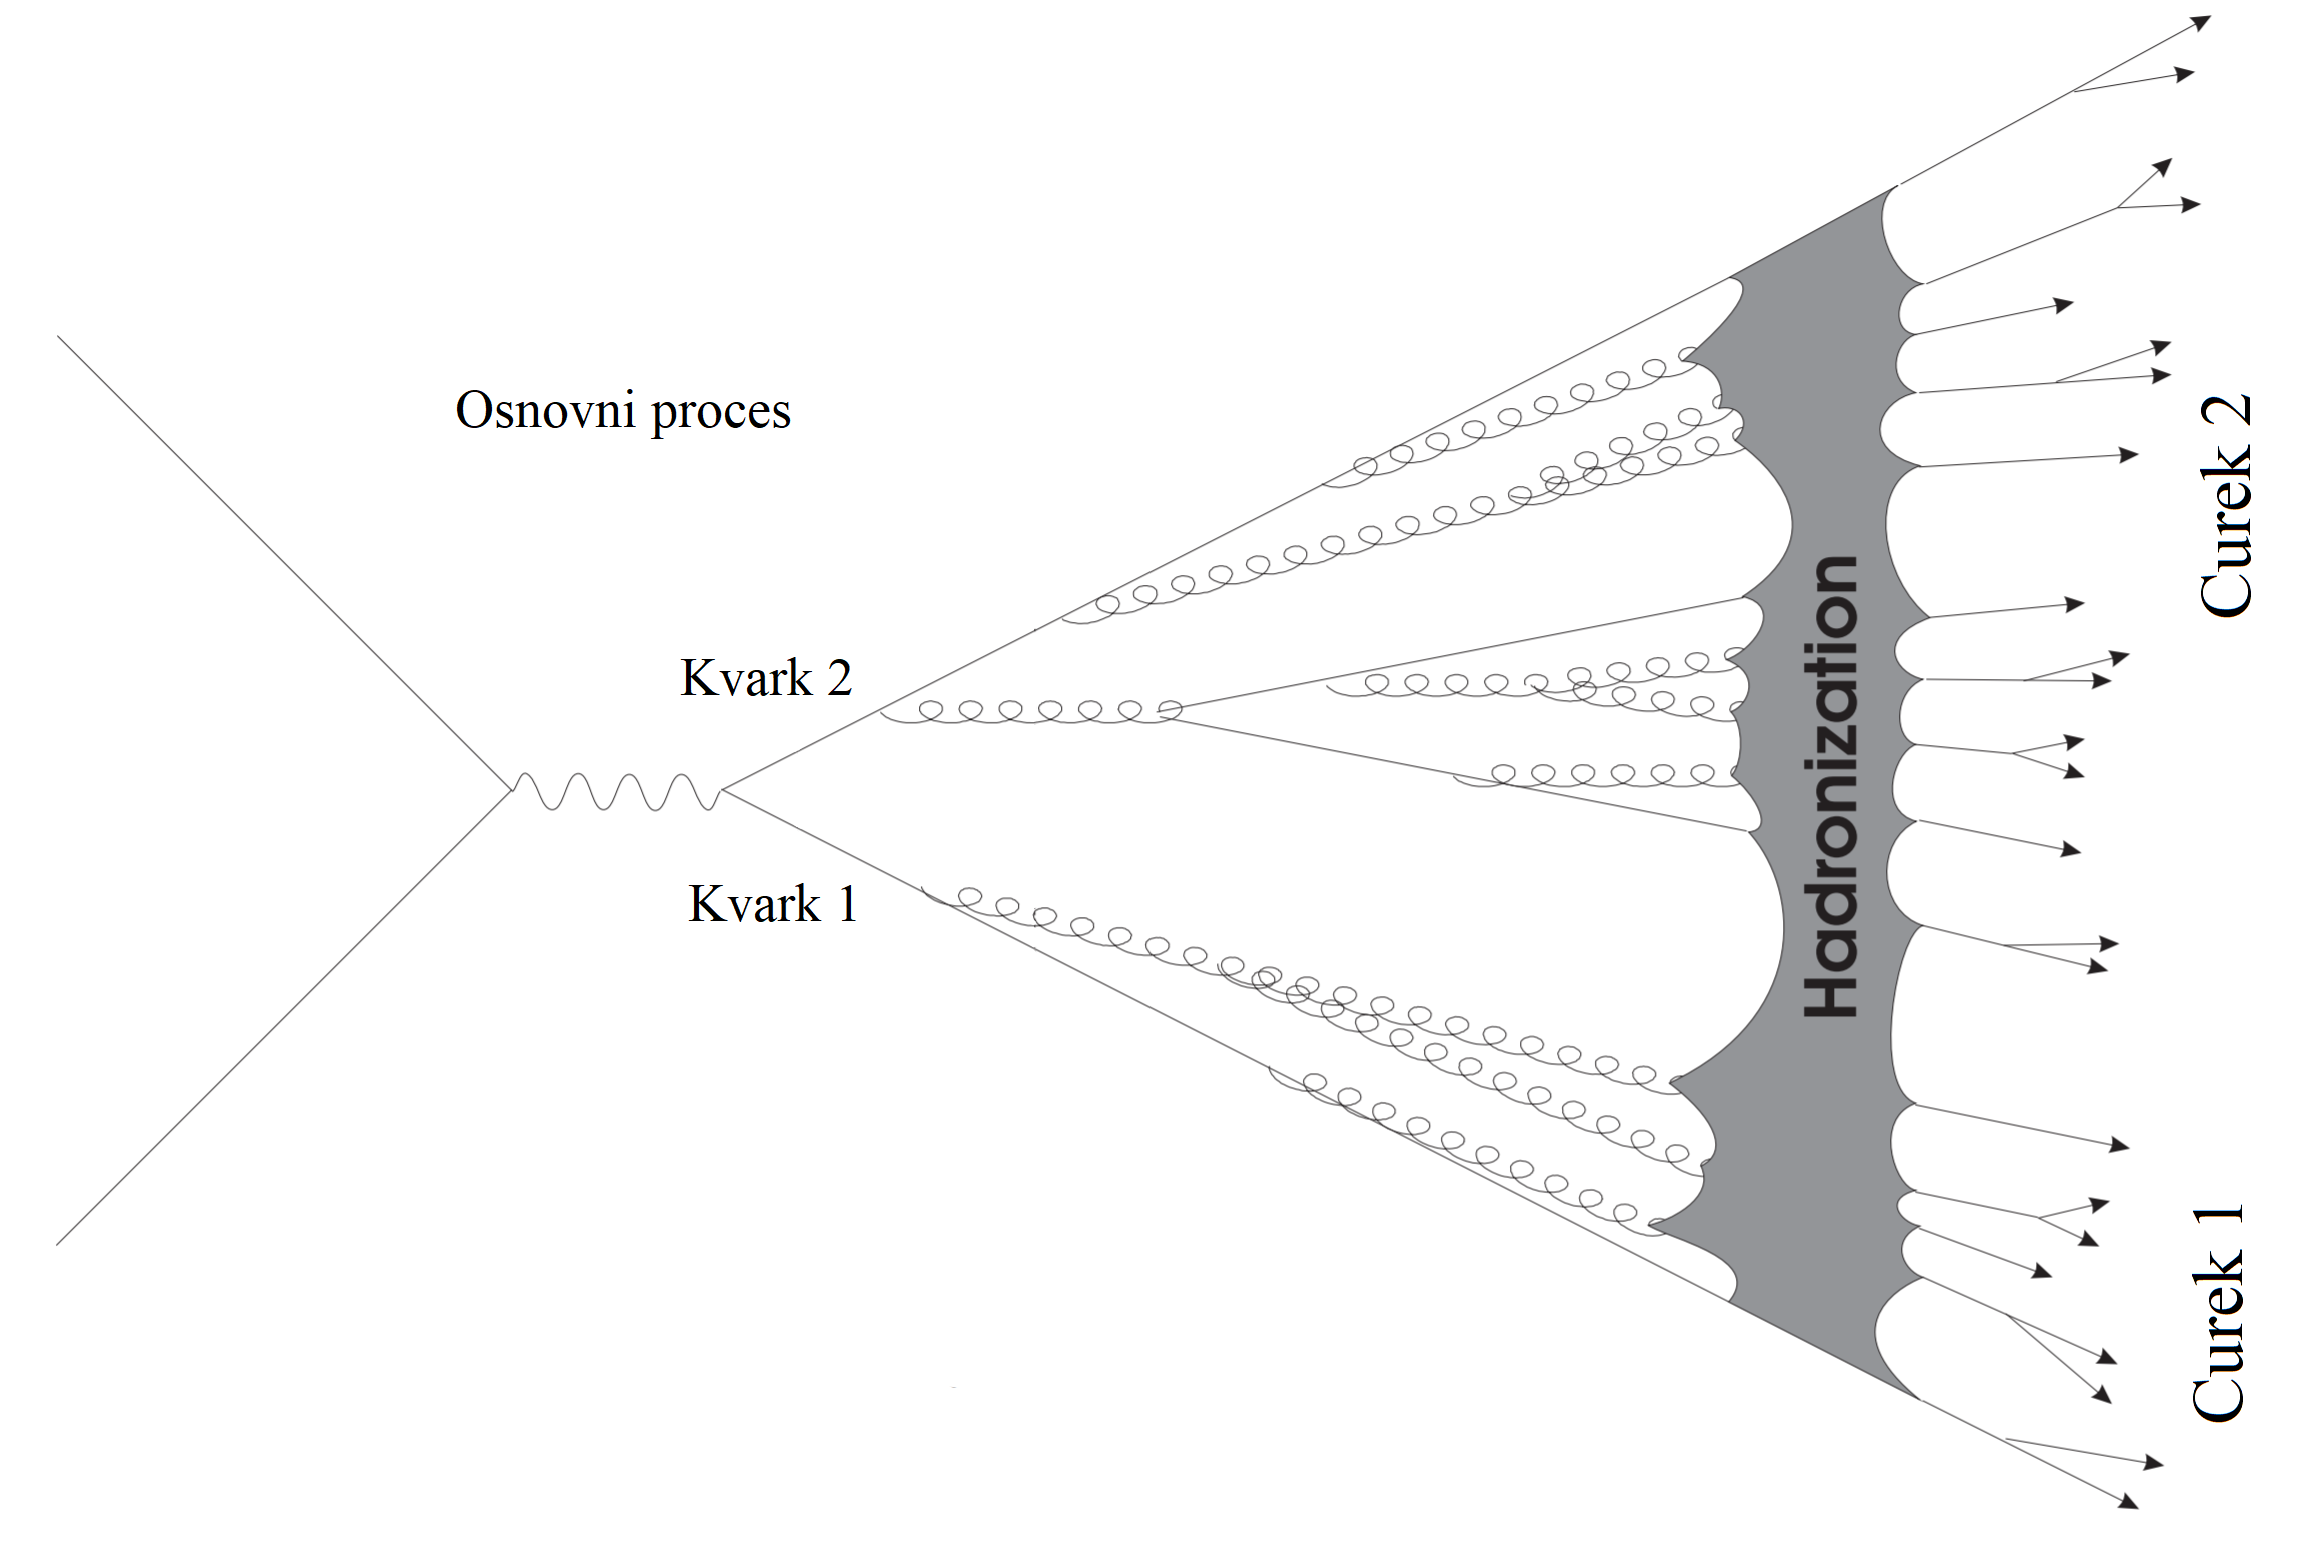
\includegraphics[width=0.8\linewidth]{hadronization-mylabels}
	\caption{Skica poteka hadronizacije iz dveh kvarkov v končnem stanju osnovnega procesa. Prirejeno iz \cite{img}.}
	\label{fig:hadronization}
\end{figure}

\subsection*{Koordinatni sistem}
Za študij kinematičnih lastnosti curkov se v visoko-energijskih trkalnikih osnovnih delcev pogosto uporablja koordinatni sistem, ki poenostavi analizo. Poljuben delec z maso $m$ v končnem stanju je mogoče opisati s četvercem gibalne količine $p = (E, \mathbf{p})$, kjer je $E = \sqrt{m^2 + |\mathbf{p}|^2}$ energija delca, $\mathbf{p}$ pa vektor gibalne količine.

\newpage
Pri visokih energijah so mase delcev pogosto zanemarljive, zato se namesto koordinat $(p_x, p_y, p_z)$ uporabljajo koordinate $(p_T, \eta, \phi)$, kjer so:

\begin{itemize}
    \item $p_T$ transverzalna gibalna količina, ki je pravokotna na smer curka,
    \item $\eta$ pseudorapidnost, ki opisuje hitrost delca neodvisno od njegove mase,
    \item $\phi$ azimutni kot.
\end{itemize}


\begin{figure}[htb]
	\centering
	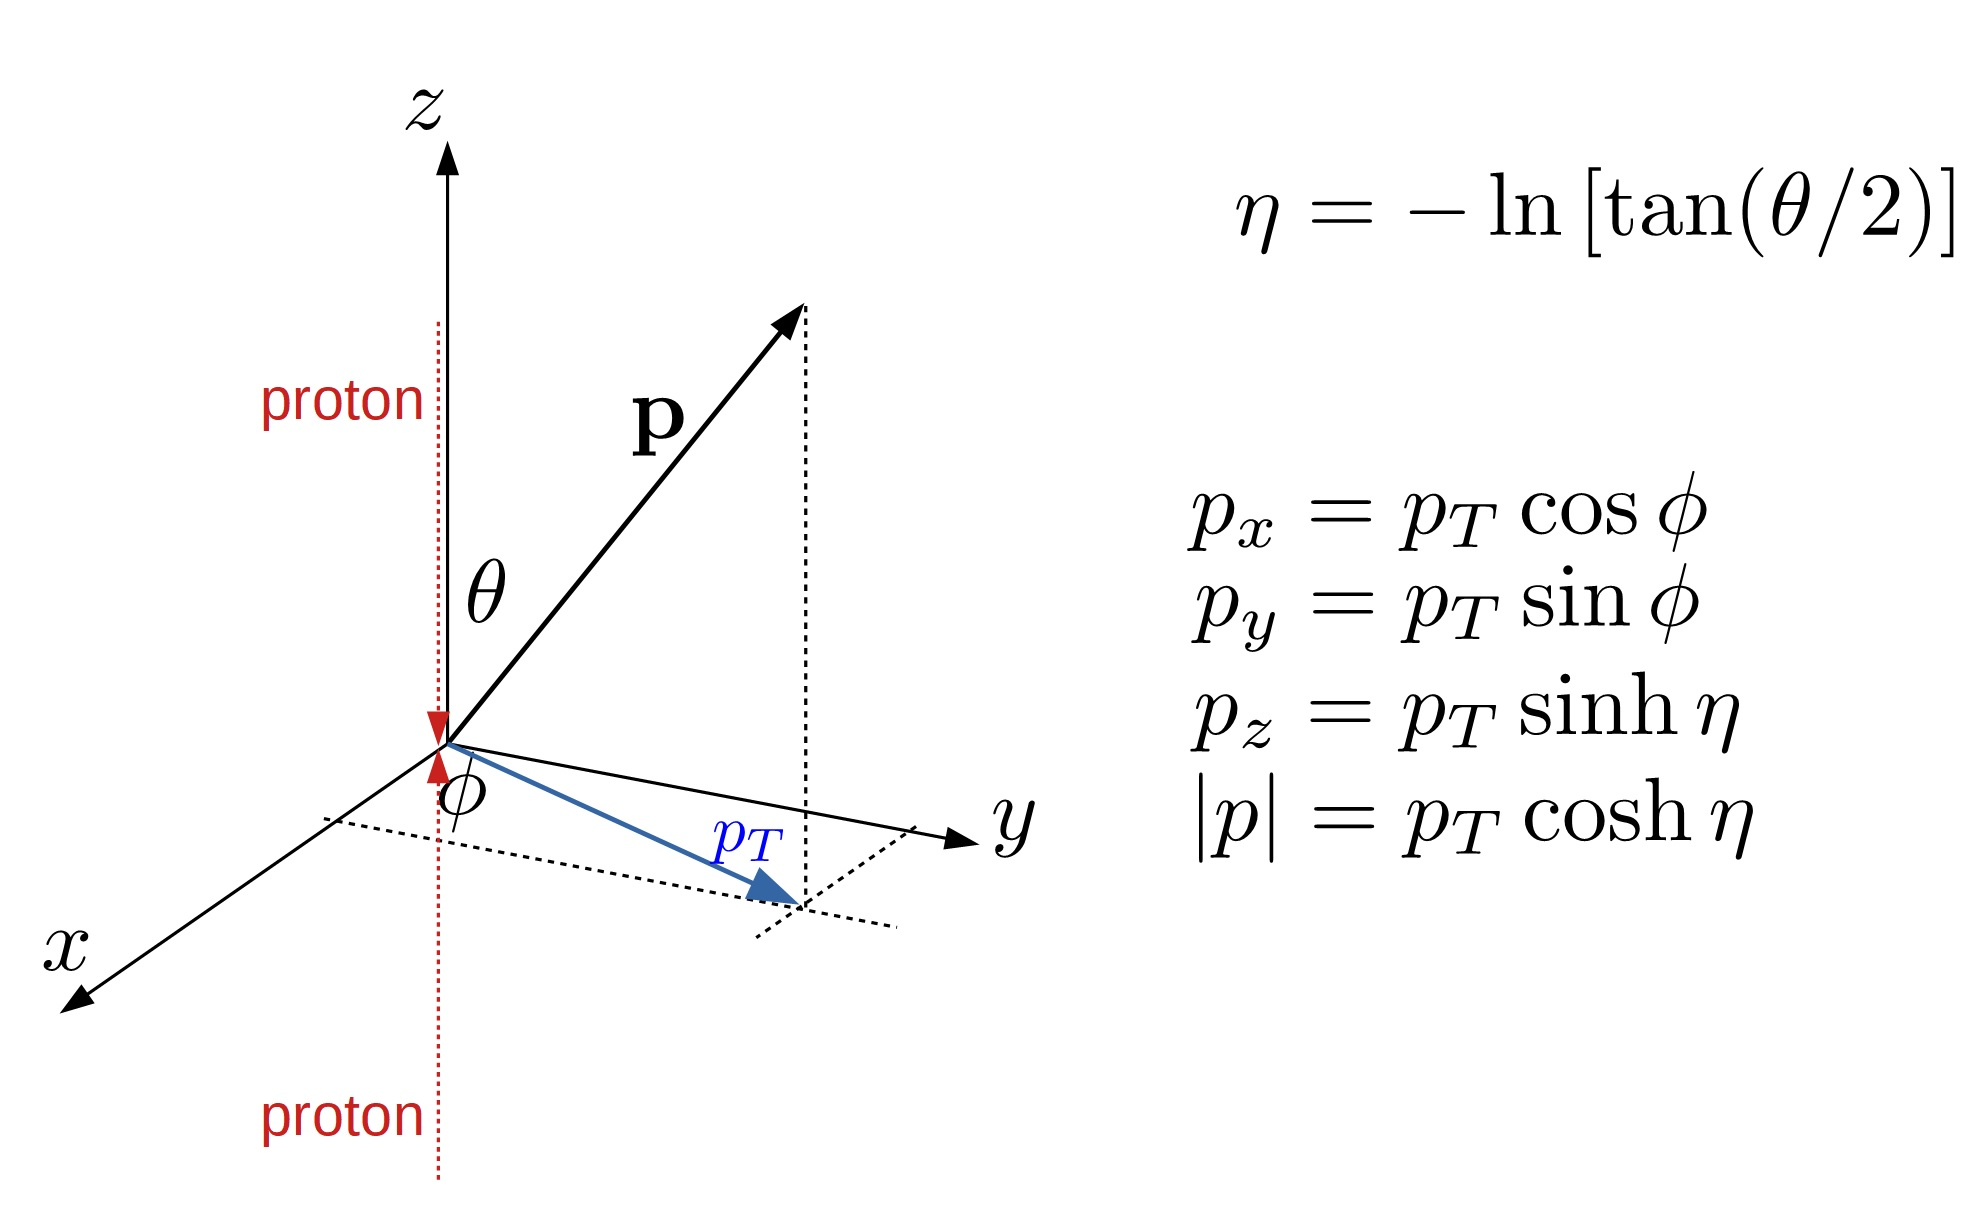
\includegraphics[width=0.8\linewidth]{collider-coordinate}
	\caption{Skica koordinatnega sistema, uporabljenega v fiziki trkalnikov osnovnih delcev in transformacija med koordinatnima sistemoma.}
	\label{fig:collider-coordinate}
\end{figure}



\section*{Algoritmi gručenja}
\label{sec:algos}
Identifikacija delcev, ki pripadajo istemu kolimiranemu hadronskemu curku, poteka z uporabo algoritmov gručenja v ravnini kotnih spremenljivk $(\eta, \phi)$. Pri tem se predvideva, da se hadroni, ki izvirajo iz skupnega osnovnega kvarka, v tej ravnini nahajajo bližje skupaj.

\subsection*{Algoritem \textit{K}-means}
Algoritem \textit{K}-means je eden najpreprostejših algoritmov gručenja.
Njegova naloga je razdeliti množico s število točk $N$ na $K$ gruč. Vsaki gruči $j=1,\dots,K$ pripada podmnožica točk in povprečje točk posamezne gruče $\mu_j$ so znana tudi kpt centroidi. Algoritem določa centroide tako, da minimizira razdaljo vsake $x_i$, kjer $i=1,\dots,N$ točke do pripadajočega centroida $\mu_j$, kjer $j=1,\dots,K$:  
\begin{equation}  
	\sum_{i=1}^{N} \|x_i-\mu_j\|^2 = \min\,.
\end{equation}  
V osnovi algoritem \textit{K}-means vključuje tri ključne korake. V prvem koraku se določijo začetne vrednosti $k$ centroidov. Te lahko izberemo z naključnim vzorčenjem znotraj ustreznih intervalov, skladnih s podatki, ali pa preprosto izberemo $k$ naključnih točk iz množice podatkov. Nato se izvede naslednja dva koraka:  
\begin{enumerate}  
	\item Na podlagi trenutnih vrednosti centroidov vsaki točki $i=1,\dots,N$ pripišemo gručo, katere centroid je najbližji (privzemi Evklidsko metriko).  
	\item Posodobimo vrednosti centroidov tako, da za vsako gruča $j$ izračunamo povprečje $\mu_j$ vseh točk, ki ji pripadajo.  
\end{enumerate}  
Ta dva koraka ponavljamo, dokler algoritem ne konvergira, tj. dokler se vrednosti centroidov med iteracijami bistveno ne prenehajo spreminjati.  

Pridobljene gruče predstavljajo curke delcev, pri čemer so vrednosti $(\eta, \phi)$ posameznega curka določene z vrednostmi pripadajočega centroida, skupna transverzalna gibalna količina gruče $p_T$ pa je izračunana kot vsota transverzalnih gibalnih količin delcev, ki pripadajo tej gruči.

Algoritem \textit{K}-means ima kljub svoji preprostosti več pomembnih slabosti. Pogosto konvergira v lokalne minimume, je izjemno občutljiv na začetno izbiro centroidov in predpostavlja, da so gruče sferične, kar lahko vodi do neustreznih rezultatov pri bolj kompleksnih podatkih. Za učinkovito uporabo tega algoritma pri gručenju curkov hadronov pa bi moral zadostiti tudi naslednjima dvema lastnostma:



\begin{enumerate}
	\item \textbf{Infrardeča varnost:} Rezultati gručenja ne smejo biti občutljivi na dodajanje novih delcev z majhno transverzalno gibalno količino.
	\item \textbf{Kolinearna varnost:} Rezultati gručenja ne smejo biti odvisni od zamenjave delca z gibalno količino $p_i$ z dvema vzporednima (kolinearnima) delcema $j$ in $k$, pri čemer velja $p_i = p_j + p_k$.
\end{enumerate}

V praksi se za identifikacijo hadronskih curkov uporabljajo algoritmi hierarhičnega gručenja.




\subsection*{Hierarhično gručenje}

V nadaljevanju so predstavljeni trije algoritmi, ki se razlikujejo po vrednosti parametra $p$, ki nastopa zgolj v eksponentu. 

Seznam delcev, ki jih izmerimo, imenujemo seznam \textit{protocurkov}. Seznam, ki ga dobimo po gručenju, imenujemo seznam \textit{pravih curkov}. Na začetku je ta seznam prazen in se polni med potekom algoritma. Algoritem vključuje prost parameter $R \sim 1$, ki je določen glede na geometrijo detektorja. Postopek gručenja je opisan v naslednjih korakih:

\begin{enumerate}
    \item Za vsak protocurek $i$ izračunamo količino $d_i = p_{T,i}^{2p}$ ter za vsak par protocurkov ($i$, $j$) izračunamo razdaljo:
    \begin{equation}
    d_{ij} = \min(p_{T,i}^{2p}, p_{T,j}^{2p}) \frac{(\eta_i - \eta_j)^2 + (\phi_i - \phi_j)^2}{R^2}.
    \end{equation}
    Pri tem glej vrednost za $(\phi_i - \phi_j)^2$ kot kvadrat kota med dvema delcema na krožnici.
    Skratka, če je $\phi_i > \phi_j$ potem je absolutna vrednost kota med delcema $\min(\phi_i - \phi_j, \phi_j + 2 \pi - \phi_i)$. Količina $\phi$ živi na mnogoterosti krožnica $S^1$ in operacija razlike ``$-$'' definirana na krožnici je drugačna kot na premici ($\mathbb{R}$).
    
    \item Poiščemo minimalno razdaljo $d_{\text{min}}$ med množicama $\{d_i\}_{i=1}^{N}$ in $\{d_{ij}\}_{i,j=1}^{N}$.
    
    \item Če je minimalna razdalja $d_{ij}$, združimo protocurka $i$ in $j$ v nov protocurek $k$, pri čemer določimo:
    \begin{equation}
    \begin{aligned}
    p_{T,k} &= p_{T,i} + p_{T,j}, \\
    \eta_k &= \frac{p_{T,i} \eta_i + p_{T,j} \eta_j}{p_{T,k}}, \\
    \phi_k &= \frac{p_{T,i} \phi_i + p_{T,j} \phi_j}{p_{T,k}}.
    \end{aligned}
    \end{equation}
    
    \item Če je minimalna razdalja $d_i$, protocurek $i$ odstranimo iz seznama protocurkov in ga vpišemo v seznam pravih curkov.
    
    \item Postopek se vrne na 1.~korak, dokler seznam protocurkov ni prazen.
\end{enumerate}

Z izbiro parametra $p \in \{-1, 0, 1\}$ (ki nastopa zgolj v eksponentu) reproduciramo znane algoritme: \textit{anti-$k_t$}, Cambridge-Aachen in $k_t$ \cite{ktEllis:1993tq, CA-Dokshitzer:1997in, antikt-Cacciari:2008gp}. Primer gručenja z vsemi tremi algoritmi je prikazan na sliki~\ref{fig:jet_areas}.



\begin{figure}[htb]
	\centering
	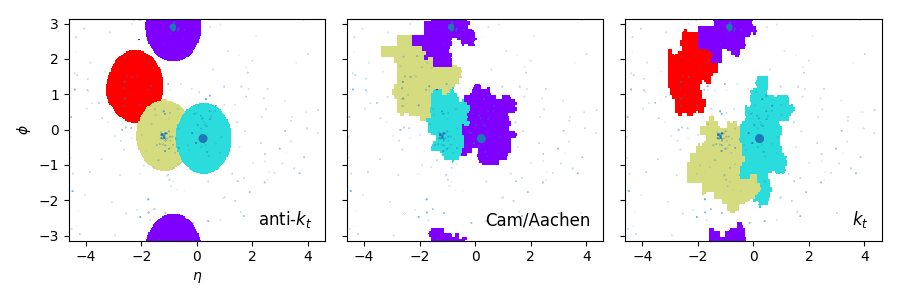
\includegraphics[width=1\linewidth]{jet_areas}
	\caption{Primer gru\v cenja v hadronske curke z algoritmi anti-$k_t$, Cambridge-Aachen in $k_t$. Delci iz dogodka so prikazani z modrimi to\v ckami, kjer ve\v cja to\v cka pomeni ve\v cji $p_T$. Obarvana podro\v cja predstavljajo curke s $p_T>10$~GeV.}
	\label{fig:jet_areas}
\end{figure}

\section*{1. del naloge}

\subsection*{Implementacija algoritmov}

\begin{enumerate}
    \item[1.] Implementiraj algoritem $K$-means po postopku, opisanem v razdelku \emph{Algoritem $K$-means} ali predstavljenem na predavanjih. Preizkusi implementacijo na priloženih podatkih v datoteki \texttt{gauss.npy}. Podatki so podani kot polje velikosti $400 \times 2$, ki predstavlja 400 delcev, pri čemer ima vsak delec dva parametra. Parametra sta naključno vzorčena iz dveh Gaussovih porazdelitev.  
    Iz najdenih gruč določi povprečne vrednosti in standardne odklone obeh Gaussovih porazdelitev.  
    Primerjaj rezultate z metodo Gaussian Mixture Model (GMM) iz knjižnice \texttt{sklearn} \cite{sklearn-gmm}.


    \item[2.] V datoteki \texttt{h\_bb\_sorted.npy} je shranjeno polje dogodkov, pri čemer vsak dogodek predstavlja trk dveh protonov, ob katerem nastane Higgsov bozon, ki razpade na dva kvarka $b$ in $\overline{b}$. Vsak dogodek vsebuje različno število delcev, katerih parametri so podani v obliki Pythonovega tupla $(p_T, \eta, \phi, m)$. Masa $m$ v tej nalogi ni pomembna. Vrednosti so simulirane z upoštevanjem efekta hadronizacije. Upoštevaj, da je geometrija cilindrična in da gručenje poteka v ravnini $(\eta, \phi)$ s periodičnimi robnimi pogoji za $\phi$.
    
    % \item[2.] V datoteki \texttt{h\_bb\_sorted.npy} je shranjen niz dogodkov, pri čemer vsak dogodek predstavlja trk dveh protonov, ob katerem nastane Higgsov bozon, ki razpade na dva kvarka $b$ in $\overline{b}$. Vsak dogodek vsebuje različno število delcev, katerih parametri so podani v obliki Pythonovega tupla $(p_T, \eta, \phi, m)$. Masa $m$ v tej nalogi ni pomembna. Vrednosti so simulirane z upoštevanjem efekta hadronizacije. {\color{red} Upoštevaj, da je geometrija cilindrična, gručenje poteka na mnogoterosti $\mathbb{R} \times S^1$, torej v ravnini ($\eta$, $\phi$) s periodičnimi robnimi pogoji za $\phi$.}

    Uporabi implementiran algoritem $K$-means na prvem dogodku iz datoteke \texttt{h\_bb\_sorted.npy} za različno število centroidov $K$. Poišči gruči z največjo transverzalno gibalno količino $p_T$, ki pripadata curkama kvarkov $b$ in $\overline{b}$. Določi četverca gibalnih količin $p_1$ in $p_2$ obeh curkov ter s tem izračunaj maso Higgsovega bozona:
    \begin{equation}
    m_h = \sqrt{(p_1 + p_2)_{\mu}(p_1 + p_2)^{\mu}} = \sqrt{(E_1 + E_2)^2 - (\mathbf{p}_1 + \mathbf{p}_2)^2}.
    \end{equation}
    Pri tem uporabi približek $E_{1,2} \approx |\mathbf{p}_{1,2}|$.
    Izmerjena masa Higgsovega bozona je 125 GeV.    

    \item[3.] Preveri, ali implementiran algoritem $K$-means zadošča infrardeči varnosti, če je uporabljen na prvem dogodku iz datoteke \texttt{h\_bb\_sorted.npy}. To pomeni, da postopoma odstranjuješ delce z najmanjšo transverzalno gibalno količino $p_T$ in spremljaš, kako se rekonstruirana masa Higgsovega bozona spreminja s številom delcev v dogodku.

    \item[4.] Implementiraj algoritem hierarhičnega gručenja in ga preizkusi na prvem dogodku.  
    Izračunaj maso Higgsovega bozona za vse tri vrednosti parametra $p \in \{-1, 0, 1\}$ in za $R = 6$. Kaj se zgodi, če povečaš ali zmanjšaš $R$? Parameter $R$ sledi lastnostim detektorja oziroma umeritvi metode na dani detektor (v praksi je fiksen).
    
    % \item[4.] Implementiraj algoritem hierarhičnega gručenja in ga testiraj na prvem dogodku.
    % Izračunaj maso Higgsovega bozona za vse tri vrednosti parametra $p = \in \{-1,0,1 \}$ in z $R = 6$. Kaj se zgodi, če povečaš ali zmanjšaš $R$? (Parameter $R$ sledi it detektorja oziroma umeritve metode na dan detektor, v praksi je fiksen)
\end{enumerate}

Implementiran algoritem hierarhičnega gručenja bo mogoče deloval zelo počasi. V praksi se za gručenje hadronskih curkov uporablja orodje FastJet \cite{fastjet-Cacciari:2011ma, opti-Cacciari:2005hq}, v katerem so algoritmi s $p \in \{-1, 0, 1\}$ optimizirani in implementirani v C++. Na voljo je tudi kot Python paket \texttt{fastjet} \cite{fastjet-python}, ki omogočajo enostavno uporabo optimiziranih algoritmov neposredno iz Python skript. Omenjeno knjižnico lahko uporabiš za preverbo svoje implementacije.

% \subsection*{Knjižnica \texttt{pyjet}}

% Implementiran algoritem hierarhičnega gručenja bo mogoče deloval zelo počasi. V praksi se za gručenje hadronskih curkov uporablja orodje \texttt{fastjet} \cite{fastjet-Cacciari:2011ma, opti-Cacciari:2005hq}, v katerem so algoritmi s $p \in \{-1, 0, 1\}$ optimizirani in implementirani v C++. Na voljo je tudi knjižnica za Python, \texttt{pyjet} \cite{pyjet}, ki omogoča enostavno uporabo optimiziranih algoritmov neposredno iz Python skript. Za uporabo algoritmov je potrebno najprej pretvoriti podatke z naslednjim ukazom:

% \begin{python}
% from pyjet import DTYPE_PTEPM, cluster
% import numpy as np

% data = np.load('h_bb_sorted.npy', allow_pickle = True)
% event = np.array(data[0], dtype=DTYPE_PTEPM) # prvi dogodek
% \end{python}

% \noindent
% Podrobnosti so opisane v dokumentaciji knjižnice \cite{pyjet}.
% Algoritem $k_t$ lahko poženemo z naslednjima ukazoma ($p=1$ za $k_t$ algoritem):


% \begin{python}
% sequence = cluster(event, ep=False, R=0.6, p=1)
% incl_jets = sequence.inclusive_jets()
% \end{python}

% \noindent
% Objekt \pyth{incl_jets} predstavlja seznam inkluzivnih curkov, kar pomeni, da so v obravnavi zajeti vsi delci iz dogodka. 
% Curki so podani v obliki objekta \pyth{PseudoJet}, s katerim lahko dostopamo, na primer, do energije $j$-tega curka z ukazom \pyth{incl_jets[j].e}, do ene od komponent gibalne količine pa z ukazom \pyth{incl_jets[j].px}.


% Za naslednje naloge uporabi algoritme iz knjižnice \pyth{pyjet}, podatke iz datoteke \texttt{h\_bb\_sorted.npy} ter postopek izračuna rekonstruirane mase Higgsovega bozona, kot je opisan v nalogi 2 (2. odstavek).



% \begin{enumerate}
% 	\setcounter{enumi}{4}
%     \item[5.\&6.] Izvedi test infrardeče varnosti za implementirani algoritem in algoritem iz knjižnice \texttt{pyjet} ter ju primerjaj (zadostuje za $p = 1$). Obenem izmeri čas izvajanja obeh algoritmov in primerjaj odvisnost časa izvajanja od števila delcev v logaritemski skali. 5.~naloga je primerjava infrardeče varnosti, medtem ko je 6.~naloga primerjava časa izvajanja.


% 	% \item[5.\&6.] Izvedi test infrardeče varnosti za implementiran algoritem in algoritem iz knjižnice 
%  %    \texttt{pyjet} ter ju primerjaj (dovolj je za $p=1$). Obenem meri čas izvajanja obeh algoritmov in primerjaj odvisnosti časa izvajanja od števila delcev v logaritemski skali. { \color{red} 5. naloga je primerjava infrardeče varnosti, medtem ko je 6. naloga primerjava časa izvajanja.}
    
    

% 	\item[7.] Poženi algoritem iz knjižnice \texttt{pyjet} na vseh dogodkih, podanih v datoteki \texttt{h\_bb.npy}, in nariši spekter rekonstruiranih invariantnih mas Higgsovega bozona. Razmisli, kako bi določil maso Higgsovega bozona skupaj s pripadajočo negotovostjo, ter ju izračunaj (zadostuje $p = 1$).

% 	% \item[7.] Poženi algoritem iz knjižnice \texttt{pyjet} na vseh dogodkih, podanih v datoteki \texttt{h\_bb.npy}, in nariši spekter rekonstruiranih invariantnih mas Higgsovega bozona. Razmisli, kako bi določil maso Higgsovega bozona skupaj s pripadajočo negotovostjo, ter ju izračunaj (dovolj je $p=1$).



% \end{enumerate}

% Če želiš vizualizirati gručenje curkov, kot je to prikazano na sliki \ref{fig:jet_areas}, si lahko pomagaš s primerom \texttt{examples/plot\_jet\_areas.py} iz repozitorija knjižnice \texttt{pyjet} \cite{pyjet}.



\section*{Označevanje curkov}

\section*{2. del naloge}

\begin{figure}[htb]
\centering
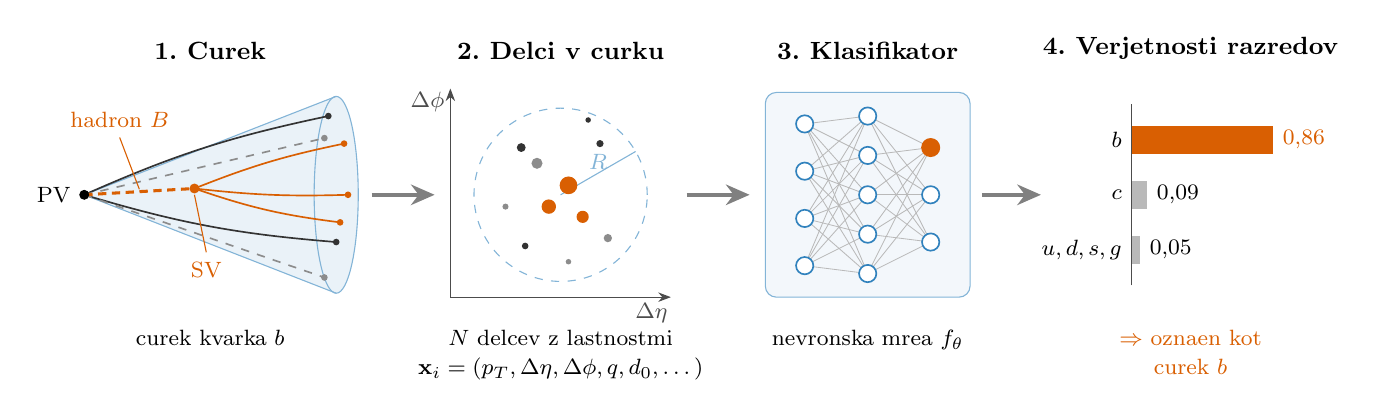
\begin{tikzpicture}[
    font=\footnotesize,
    naslov/.style={font=\small\bfseries, anchor=south},
    opis/.style={anchor=north, align=center},
    sled/.style={line width=0.6pt, black!80},
    bsled/.style={line width=0.6pt, bcol},
    nevtr/.style={line width=0.6pt, neucol, dashed},
    tok/.style={-{Stealth[length=3mm,width=2.6mm]}, line width=1.4pt, black!50},
  ]
  % ---------- 1. Curek ----------
  \begin{scope}
    \fill[jetcol!10] (0,0) -- (3.2,1.25) arc[start angle=90, end angle=-90, x radius=0.28, y radius=1.25] -- cycle;
    \draw[jetcol!60] (0,0) -- (3.2,1.25) (0,0) -- (3.2,-1.25);
    \draw[jetcol!60] (3.2,0) ellipse[x radius=0.28, y radius=1.25];
    % sledi iz primarnega verteksa
    \draw[sled] (0,0) to[bend left=6] (3.1,1.0);
    \draw[sled] (0,0) to[bend right=6] (3.2,-0.6);
    \draw[nevtr] (0,0) -- (3.05,-1.05);
    \draw[nevtr] (0,0) -- (3.05,0.72);
    % hadron B in sekundarni verteks
    \draw[bcol, line width=1.1pt, densely dashed] (0,0) -- (1.4,0.08);
    \draw[bsled] (1.4,0.08) to[bend left=5] (3.3,0.65);
    \draw[bsled] (1.4,0.08) to[bend right=4] (3.35,0.0);
    \draw[bsled] (1.4,0.08) to[bend right=6] (3.25,-0.35);
    \foreach \p in {(3.1,1.0),(3.2,-0.6)} \fill[black!80] \p circle (1.2pt);
    \foreach \p in {(3.05,-1.05),(3.05,0.72)} \fill[neucol] \p circle (1.2pt);
    \foreach \p in {(3.3,0.65),(3.35,0.0),(3.25,-0.35)} \fill[bcol] \p circle (1.2pt);
    \fill (0,0) circle (1.8pt);
    \fill[bcol] (1.4,0.08) circle (1.8pt);
    \node[left] at (-0.05,0) {PV};
    \node[bcol] (sv) at (1.55,-0.95) {SV};
    \draw[bcol, thin] (sv.north) -- (1.4,0.0);
    \node[bcol] (bh) at (0.45,0.95) {hadron $B$};
    \draw[bcol, thin] (bh.south) -- (0.7,0.07);
    \node[naslov] at (1.6,1.6) {1.~Curek};
    \node[opis] at (1.6,-1.6) {curek kvarka $b$};
  \end{scope}

  \draw[tok] (3.65,0) -- (4.45,0);

  % ---------- 2. Delci v curku ----------
  \begin{scope}[xshift=4.65cm]
    \draw[-{Stealth[length=1.6mm]}, black!70] (0,-1.3) -- (2.8,-1.3) node[below left, inner sep=1pt, yshift=-1pt] {$\Delta\eta$};
    \draw[-{Stealth[length=1.6mm]}, black!70] (0,-1.3) -- (0,1.35) node[below left, inner sep=1pt, xshift=-1pt] {$\Delta\phi$};
    \draw[jetcol!60, dashed] (1.4,0) circle (1.1);
    \draw[jetcol!60] (1.4,0) -- node[above, inner sep=1pt] {$R$} ++(30:1.1);
    % nevtralni delci
    \foreach \x/\y/\r in {1.1/0.4/2.0, 2.0/-0.55/1.5, 0.7/-0.15/1.1, 1.5/-0.85/1.0}
      \fill[neucol] (\x,\y) circle (\r pt);
    % nabiti delci iz PV
    \foreach \x/\y/\r in {0.9/0.6/1.6, 1.9/0.65/1.3, 0.95/-0.65/1.2, 1.75/0.95/1.0}
      \fill[black!80] (\x,\y) circle (\r pt);
    % delci iz razpada hadrona B
    \foreach \x/\y/\r in {1.5/0.12/3.2, 1.25/-0.15/2.6, 1.68/-0.28/2.2}
      \fill[bcol] (\x,\y) circle (\r pt);
    \node[naslov] at (1.4,1.6) {2.~Delci v curku};
    \node[opis] at (1.4,-1.6) {$N$ delcev z lastnostmi\\[1pt]$\mathbf{x}_i = (p_T, \Delta\eta, \Delta\phi, q, d_0, \dots)$};
  \end{scope}

  \draw[tok] (7.65,0) -- (8.45,0);

  % ---------- 3. Klasifikator ----------
  \begin{scope}[xshift=8.65cm]
    \draw[rounded corners=4pt, fill=jetcol!6, draw=jetcol!60] (0,-1.3) rectangle (2.6,1.3);
    \foreach \i/\y in {1/-0.9,2/-0.3,3/0.3,4/0.9} \coordinate (a\i) at (0.5,\y);
    \foreach \i/\y in {1/-1.0,2/-0.5,3/0,4/0.5,5/1.0} \coordinate (b\i) at (1.3,\y);
    \foreach \i/\y in {1/-0.6,2/0,3/0.6} \coordinate (c\i) at (2.1,\y);
    \foreach \i in {1,...,4} \foreach \j in {1,...,5} \draw[gray!55, line width=0.3pt] (a\i) -- (b\j);
    \foreach \i in {1,...,5} \foreach \j in {1,...,3} \draw[gray!55, line width=0.3pt] (b\i) -- (c\j);
    \foreach \p in {a1,a2,a3,a4,b1,b2,b3,b4,b5,c1,c2}
      \filldraw[fill=white, draw=jetcol, line width=0.6pt] (\p) circle (0.11);
    \filldraw[fill=bcol, draw=bcol, line width=0.6pt] (c3) circle (0.11);
    \node[naslov] at (1.3,1.6) {3.~Klasifikator};
    \node[opis] at (1.3,-1.6) {nevronska mreža $f_\theta$\\[1pt]};
  \end{scope}

  \draw[tok] (11.4,0) -- (12.15,0);

  % ---------- 4. Verjetnosti razredov ----------
  \begin{scope}[xshift=12.3cm]
    \fill[bcol] (1.0,0.52) rectangle ++(1.8,0.36);
    \fill[gray!55] (1.0,-0.18) rectangle ++(0.20,0.36);
    \fill[gray!55] (1.0,-0.88) rectangle ++(0.11,0.36);
    \draw[black!70] (1.0,-1.15) -- (1.0,1.15);
    \node[left] at (1.0,0.7) {$b$};
    \node[left] at (1.0,0.0) {$c$};
    \node[left] at (1.0,-0.7) {$u,d,s,g$};
    \node[right, bcol] at (2.8,0.7) {$0{,}86$};
    \node[right] at (1.20,0.0) {$0{,}09$};
    \node[right] at (1.11,-0.7) {$0{,}05$};
    \node[naslov] at (1.75,1.6) {4.~Verjetnosti razredov};
    \node[opis, bcol] at (1.75,-1.6) {$\Rightarrow$ označen kot\\[1pt]curek $b$};
  \end{scope}
\end{tikzpicture}
\caption{Shematski prikaz označevanja curkov. (1)~V curku kvarka $b$ hadron $B$ preleti nekaj milimetrov, preden razpade v sekundarnem verteksu (SV), ki je premaknjen od primarnega verteksa (PV) trka. Polne črte so sledi nabitih delcev (ukrivljene v magnetnem polju), črtkane pa nevtralni delci. (2)~Curek predstavimo kot neurejeno množico (oblak) $N$ delcev v ravnini $(\Delta\eta, \Delta\phi)$ glede na os curka. Velikost točke ustreza $p_T$ delca, krožnica pa radiju curka $R$. Vsak delec opišemo z vektorjem lastnosti $\mathbf{x}_i$, npr.\ z nabojem $q$ in vpadnim parametrom sledi $d_0$. (3)~Klasifikator, npr.\ nevronska mreža, (4)~vrne verjetnosti $p_k$, da curek izvira iz razreda $k$, pri čemer velja $\sum_k p_k = 1$. Curek označimo z najverjetnejšim razredom.}
\label{fig:tagging}
\end{figure}

\newpage

\begin{thebibliography}{10}
\bibitem{pdg}
Particle Data Group, pdgLive, \url{https://pdglive.lbl.gov/Viewer.action}.
\bibitem{jetsSeymour:1995gq}
M.~H. Seymour, ``Jets in QCD'', AIP Conf. Proc. 357 (1996) 568--587, \href{https://arxiv.org/abs/hep-ph/9506421}{arXiv:hep-ph/9506421}.
\bibitem{jetbook}
A.~Banfi, ``Introduction'', v: Hadronic Jets, Morgan and Claypool Publishers (2016), str. 1-1 -- 1-12, \href{https://doi.org/10.1088/978-1-6817-4073-7ch1}{doi:10.1088/978-1-6817-4073-7ch1}.
\bibitem{img}
D.~Buskulic \emph{et al.}, ``Measurement of $\alpha_s$ from scaling violations in fragmentation functions in $e^+e^-$ annihilation'' (1995).
\bibitem{ktEllis:1993tq}
S.~D. Ellis, D.~E. Soper, ``Successive combination jet algorithm for hadron collisions'', Phys. Rev. D 48 (1993) 3160--3166, \href{https://arxiv.org/abs/hep-ph/9305266}{arXiv:hep-ph/9305266}.
\bibitem{CA-Dokshitzer:1997in}
Y.~L. Dokshitzer, G.~Leder, S.~Moretti, B.~Webber, ``Better jet clustering algorithms'', JHEP 08 (1997) 001, \href{https://arxiv.org/abs/hep-ph/9707323}{arXiv:hep-ph/9707323}.
\bibitem{antikt-Cacciari:2008gp}
M.~Cacciari, G.~P. Salam, G.~Soyez, ``The anti-$k_t$ jet clustering algorithm'', JHEP 04 (2008) 063, \href{https://arxiv.org/abs/0802.1189}{arXiv:0802.1189}.
\bibitem{sklearn-gmm}
scikit-learn, dokumentacija razreda \texttt{GaussianMixture}, \url{https://scikit-learn.org/stable/modules/generated/sklearn.mixture.GaussianMixture.html}.
\bibitem{fastjet-Cacciari:2011ma}
M.~Cacciari, G.~P. Salam, G.~Soyez, ``FastJet User Manual'', Eur. Phys. J. C 72 (2012) 1896, \href{https://arxiv.org/abs/1111.6097}{arXiv:1111.6097}.
\bibitem{opti-Cacciari:2005hq}
M.~Cacciari, G.~P. Salam, ``Dispelling the $N^{3}$ myth for the $k_t$ jet-finder'', Phys. Lett. B 641 (2006) 57--61, \href{https://arxiv.org/abs/hep-ph/0512210}{arXiv:hep-ph/0512210}.
\bibitem{fastjet-python}
Scikit-HEP, \texttt{fastjet}: FastJet paket za Python in Awkward Array, \url{https://github.com/scikit-hep/fastjet}, dokumentacija: \url{https://fastjet.readthedocs.io/en/latest/}.
\bibitem{ParT}
H.~Qu, C.~Li, S.~Qian, ``Particle Transformer for Jet Tagging'', Proceedings of the 39th International Conference on Machine Learning (ICML), PMLR 162 (2022) 18281--18292, \href{https://arxiv.org/abs/2202.03772}{arXiv:2202.03772}.

\end{thebibliography}

\end{document}